\newif\ifaastex
\IfFileExists{aastex631.cls}{%
  \aastextrue
  \documentclass[twocolumn]{aastex631}
}{%
  \aastexfalse
  \documentclass[twocolumn]{article}
  \usepackage[margin=0.75in]{geometry}
  \usepackage[authoryear]{natbib}
  \usepackage{graphicx}
  \newcommand{\shorttitle}[1]{}
  \newcommand{\shortauthors}[1]{}
  \newcommand{\affiliation}[1]{}
  \newcommand{\correspondingauthor}[1]{}
  \newcommand{\email}[1]{}
  \newcommand{\keywords}[1]{\par\noindent\textbf{Keywords: }##1\par}
  \newcommand{\acknowledgments}{\section*{Acknowledgments}}
  \newcommand{\software}[1]{\section*{Software}##1}
}

\usepackage{amsmath}
\usepackage{booktabs}
\usepackage[hidelinks]{hyperref}

\graphicspath{{figs/boss_completion/}}

\shorttitle{ECHOES for BOSS CMASS-South}
\shortauthors{Abel et al.}

\begin{document}

\title{\textsc{ECHOES}: Equal-weight Completed Hypothetical Observation Ensembles
for BOSS CMASS-South:
Survey-Ready Posterior Samples for Arbitrary Galaxy-Clustering Statistics}

\author{Tom Abel}
\affiliation{Kavli Institute for Particle Astrophysics and Cosmology, Stanford University, Stanford, CA, USA}
\correspondingauthor{Tom Abel}
\email{tabel@stanford.edu}

\ifaastex\else\maketitle\fi

\begin{abstract}
Most precision galaxy-clustering analyses communicate between survey teams and
theory teams through a small set of summary statistics, most often two-point
correlation functions or power spectra.  This convention is powerful because the
observational effects that enter these statistics have been studied for decades,
but it also makes each new statistic responsible for reinterpreting the survey
window, fiber assignment, redshift failures, imaging systematics, and random
catalogs.  We present \textsc{ECHOES}, Equal-weight Completed Hypothetical
Observation Ensembles, for BOSS DR12 CMASS-South: an ensemble of equal-weight,
cosmology-free completed catalogs that keep every
observed galaxy at its measured $(\alpha,\delta,z)$ and restore the
spectroscopically missing galaxies at their real SDSS imaging positions.  The
unknown redshifts are sampled from a data-driven posterior combining a
color-space $k$-nearest-neighbor photo-$z$, an empirical close-pair prior, and a
local-density line-of-sight prior.  Smooth imaging-systematic weights are
represented by local analog galaxies rather than by per-object completeness
weights.  The released posterior is compact: one 2.04 MB file stores the fixed
observed catalog and the inverse CDF for each restored target, and a
numpy-only sampler generates reproducible complete catalogs from integer seeds.
For seed 0 the sample contains 119,923 equal-weight galaxies, of which 109,636
are observed, 5,272 are restored fiber-collision targets, 1,505 are restored
redshift failures, and 3,510 are imaging-systematic analogs.  We validate the
product against truth-known completions and MultiDark-Patchy mocks, finding
that projected clustering is recovered to the 1--2\% level over
$0.5<r_p<40\,h^{-1}{\rm Mpc}$, while the posterior completion uncertainty in
$w_p(r_p)$ is only 0.17--0.44\% per bin, below the sample-variance scale of the
BOSS South Galactic Cap.  We also describe a fully complementary graphGP route:
a conditional anisotropic Gaussian-process posterior over the galaxy density
field, sampled by Matheron's rule on a sparse graph and evaluated along each
missing galaxy's line of sight.  The resulting catalogs are intended to let
analysts run two-point, higher-order, marked, nearest-neighbor, topological,
field-level, or simulation-based statistics directly on survey-ready data while
propagating the observational-completion uncertainty by resampling the catalog
posterior.
\end{abstract}

\keywords{Large-scale structure of the universe (902); Galaxy surveys (598);
Astrostatistics (1882); Cosmological parameters (339); Observational cosmology
(1146)}

\section{Introduction}
\label{sec:intro}

The central compression in observational large-scale structure is not a
simulation or an estimator, but an agreement about what object is being
communicated.  A survey team measures a summary statistic from a complicated
instrumental and astrophysical selection function; a theory team predicts the
same statistic for a cosmological and galaxy-formation model.  The summary
statistic is the interface.  For modern spectroscopic galaxy surveys that
interface has usually been a two-point statistic: a correlation function, a
projected correlation function, a redshift-space multipole, or a Fourier-space
power spectrum \citep{DavisPeebles1983,LandySzalay1993,Hamilton1993,FKP1994}.
This choice is not merely historical.  The observational corrections for
two-point clustering have been revisited repeatedly, calibrated in mocks, and
encoded in survey catalogs, random catalogs, and weights.

At the same time, the cosmological information in a galaxy survey is not
exhausted by two-point clustering.  The literature contains a long sequence of
proposed and demonstrated summaries: higher-order moments and hierarchical
statistics \citep{SzapudiSzalay1993,FryGaztanaga1993}, void-probability
functions \citep{Einasto1991}, counts-in-cells and one-point density PDFs
\citep{Baugh1995,Szapudi1996,Uhlemann2020,Friedrich2020}, marked correlation
functions and marked power spectra \citep{Harker2006,Satpathy2019,Massara2021,
Massara2023}, nearest-neighbor distributions \citep{BanerjeeAbel2021,Yuan2024},
wavelet and scattering-transform statistics \citep{Cheng2020,Valogiannis2022,
Regaldo2024}, persistent-homology summaries of the cosmic web
\citep{Wilding2021,Biagetti2022,Yip2024}, and field-level or
simulation-based inference methods \citep{JascheWandelt2013,Nguyen2024,
Lemos2024,Hahn2023Mock,Hahn2023PNAS,Hahn2024NatAs,Hahn2024Bispectrum,
Massara2025SBI}.  Large simulation suites such as Quijote
\citep{Quijote2020} have been essential for calibrating and stress-testing
many of these summaries.  The Beyond-2pt Collaboration's parameter-masked mock-data
challenge \citep{Beyond2pt2025} makes the same point in a deliberately broad
form: once the Gaussian, two-point description is relaxed, many summaries can
extract complementary information, and their relative utility is an empirical
question.

The barrier between those ideas and real spectroscopic data is often not the
statistic itself.  It is the observational model.  A statistic that is easy to
define on a periodic simulation box can become difficult to interpret in a
survey with angular holes, variable targeting, fiber collisions, redshift
failures, stellar density, seeing, extinction, and redshift-dependent selection.
For two-point statistics, decades of work have made the corresponding
correction pathways usable.  For many newer statistics, the same corrections
are either rederived from scratch, approximated, or avoided by restricting the
analysis to mocks and forecasts.  This paper asks whether the interface can be
moved one step earlier: instead of releasing only weighted galaxies and
randoms and asking every statistic to understand the weights, release a
posterior over completed galaxy catalogs that have already absorbed the main
observational incompleteness into equal-weight point sets.

This perspective has a long historical lineage.  The first large maps of
extragalactic structure already had to confront the fact that the sky is not a
uniform observing surface.  \citet{Hubble1934} discussed the distribution of
extragalactic nebulae in the presence of Galactic obscuration, a problem that
later became a quantitative dust-correction program culminating in all-sky
reddening maps such as \citet{SFD1998}.  Redshift surveys then turned angular
inhomogeneity into a three-dimensional selection problem
\citep{DavisPeebles1983,deLapparent1986}.  The 2dF Galaxy Redshift Survey and
SDSS established the modern industrial mode of galaxy redshift surveys
\citep{York2000,Colless2001,Cole2005}, and the SDSS luminous red galaxy sample
made the two-point correlation function a precision cosmological observable
with the detection of the baryon acoustic feature \citep{Eisenstein2005}.

BOSS inherited this history and made it operational.  Its spectrographs,
fiber system, target selection, and large-scale-structure catalogs are
documented in \citet{Dawson2013,Smee2013,Reid2016}.  The final DR12 cosmology
analyses used a mature system of angular masks, radial random catalogs,
redshift-failure weights, close-pair weights, imaging-systematic weights, and
FKP weights \citep{Alam2017,Ross2017}.  The resulting measurements were robust
because the effect of these ingredients on the two-point statistics had been
studied.  But the same survey artifacts have no reason to couple only to
two-point functions.  Fiber collisions remove close angular pairs; redshift
failures correlate with observing conditions and target properties; imaging
systematics modulate the target density across degree scales; and the random
catalog carries a particular representation of the angular and radial selection
function.

The same issues will not become simpler in later surveys.  DESI's robotic
fiber-positioner system and its fiber-assignment algorithm create a richer
assignment problem than the BOSS plug-plate geometry
\citep{Silber2023,Pinol2017,Lan2023,Lasker2025}.  Euclid, the Nancy Grace
Roman Space Telescope, the Chinese Space Station Telescope, and the Vera C.
Rubin Observatory's LSST will produce enormous galaxy samples with their own
mixtures of imaging, spectroscopy, selection, and calibration systematics
\citep{Euclid2025,Wang2022,Miao2023,CSST2026,ZhanTyson2018}.  If those surveys
wish to serve a community that will analyze the data with statistics not yet
standardized, the most useful data product may not be a single corrected
summary statistic.  It may be a survey-ready probabilistic catalog.

This work builds such a product for BOSS DR12 CMASS-South.  We call the
approach \textsc{ECHOES}: Equal-weight Completed Hypothetical Observation
Ensembles, echoes of the survey one would have taken if the principal
spectroscopic incompleteness and smooth imaging systematics were negligible.
It is not a new cosmological measurement.  It is a data-modeling and validation
paper.  We construct an ensemble of completed catalogs conditioned on the
published BOSS data and SDSS imaging: observed spectroscopic galaxies remain
fixed, missing targets are restored at real imaging positions, and redshift
uncertainty is sampled.  The ensemble is cosmology-free in the sense that it
contains only RA, Dec, and redshift; an analyst chooses a fiducial cosmology
only when measuring three-dimensional clustering.  The ECHOES product is
designed so that the summary statistic, rather than the observational
correction, can once again be the object under study.

\section{ECHOES Completed-Survey Methodology}
\label{sec:method}

\subsection{Data model and scope}
\label{subsec:datamodel}

The target ECHOES product is an ensemble
\begin{equation}
  {\cal C}^{(s)} =
  \{ \alpha_i^{(s)},\delta_i^{(s)},z_i^{(s)},p_i^{(s)} \}_{i=1}^{N_s},
  \label{eq:catalog}
\end{equation}
where $s$ is a seed and $p_i$ is a provenance code.  The coordinates are
observed RA, Dec, and redshift.  No comoving coordinate, Alcock--Paczynski
scaling \citep{AlcockPaczynski1979}, redshift-space model \citep{Kaiser1987},
or fiducial cosmology is stored in the catalog.  The completion posterior is
conditional on the observed BOSS catalog, the SDSS imaging target catalog, and
the BOSS angular mask and weights.  It does not represent cosmic variance; it
represents the uncertainty in replacing spectroscopic incompleteness and smooth
imaging-systematic weights by equal-weight galaxies.

The ECHOES product corrects three effects in the default release: fiber collisions,
redshift failures, and the smooth imaging-systematic modulation represented by
\texttt{WEIGHT\_SYSTOT}.  An optional inpainted version also fills interior mask
holes, but the default scientific product leaves the survey mask explicit.  The
FKP weight \citep{FKP1994} is not a completeness correction and is not converted
into galaxies.  Analysts may still apply FKP or other inverse-variance weights
when estimating a statistic; the released point catalog itself is equal weight.

\subsection{BOSS CMASS-South sample}
\label{subsec:bossdata}

We use the BOSS DR12 CMASS South Galactic Cap subset with the same clean cuts
used in several modern analyses of these data:
\begin{equation}
  {\rm RA}<28^\circ \; {\rm or} \; {\rm RA}>335^\circ,\qquad
  {\rm Dec}>-6^\circ,\qquad
  0.45<z<0.60 .
\end{equation}
The input contains 109,636 observed spectroscopic galaxies.  The BOSS
completeness weights imply a mean completeness correction of 1.074, or about
7.4\% missing objects before the smooth imaging-systematic analog step.  In the
real target recovery used here, 5,272 fiber-collision targets and 1,505
redshift-failure targets are restored, for 6,777 spectroscopically missing
galaxies in the compact posterior package.

The BOSS loader reads the standard large-scale-structure columns
\texttt{RA}, \texttt{DEC}, \texttt{Z}, \texttt{WEIGHT\_SYSTOT},
\texttt{WEIGHT\_NOZ}, \texttt{WEIGHT\_CP}, and \texttt{WEIGHT\_FKP}.  It also
reads \texttt{MODELFLUX}, \texttt{EXTINCTION}, \texttt{IMATCH}, and
\texttt{ICOLLIDED} when photometry is requested.  Extinction-corrected
Pogson magnitudes are computed as
\begin{equation}
  m_b = 22.5 - 2.5\log_{10} f_b - A_b,
\end{equation}
with adjacent colors $(u-g,g-r,r-i,i-z)$.  The photometric-redshift model uses
$(g-r,r-i,i-z,i)$, dropping the $u$ band because it is noisy for the red CMASS
population.

\subsection{Recovering the missing target list}
\label{subsec:targets}

The completion uses real imaging positions for missing galaxies.  We start
from the DR12 CMASS color-selected target catalog, cross-matched to the good
redshift BOSS LSS catalog.  A target with a spectrum but nonzero
\texttt{ZWARNING} is classified as a redshift failure.  A target with no usable
spectrum is eligible to be a fiber-collision target.  Because the no-spectrum
photometric pool also contains objects that were not part of the final BOSS LSS
sample, it is tied back to the BOSS bookkeeping.  For each observed survivor
with \texttt{WEIGHT\_CP}$>1$, the algorithm greedily claims
$\mathrm{round}(\texttt{WEIGHT\_CP}-1)$ nearest unclaimed no-spectrum targets
within the BOSS fiber-collision scale, $62''$.  Redshift failures are tied to
survivors with \texttt{WEIGHT\_NOZ}$>1$ using the analogous
$\mathrm{round}(\texttt{WEIGHT\_NOZ}-1)$ count and a wider $15'$ neighborhood.
This preserves the integer count implied by the official weights while
placing the restored galaxies at their actual imaging positions and colors.

\subsection{Color-space photo-\texorpdfstring{$z$}{z} posterior}
\label{subsec:photoz}

For each missing target we require a redshift posterior, not only a point
estimate.  We fit a nonparametric $k$-nearest-neighbor model to the observed
CMASS galaxies in the whitened four-dimensional feature space
$(g-r,r-i,i-z,i)$.  The default model uses $k=100$ and a \texttt{cKDTree}.  For a
query feature vector ${\bf x}$, the posterior support is the set of neighbor
redshifts $\{z_j\}_{j=1}^k$ with inverse-distance weights
\begin{equation}
  w_j({\bf x}) =
  \frac{(d_j^2+\epsilon)^{-1}}
       {\sum_{\ell=1}^k(d_\ell^2+\epsilon)^{-1}} .
\end{equation}
The held-out diagnostic in the report gives
$\sigma_{\rm NMAD}=0.019$, a bias of $-0.0006$, a catastrophic outlier rate of
1.8\%, and a probability-integral-transform mean of 0.503.  These numbers are
adequate for the role the photo-$z$ plays here: it supplies a color likelihood
that is then multiplied by a local-density prior along the same line of sight.

\begin{figure*}
\centering
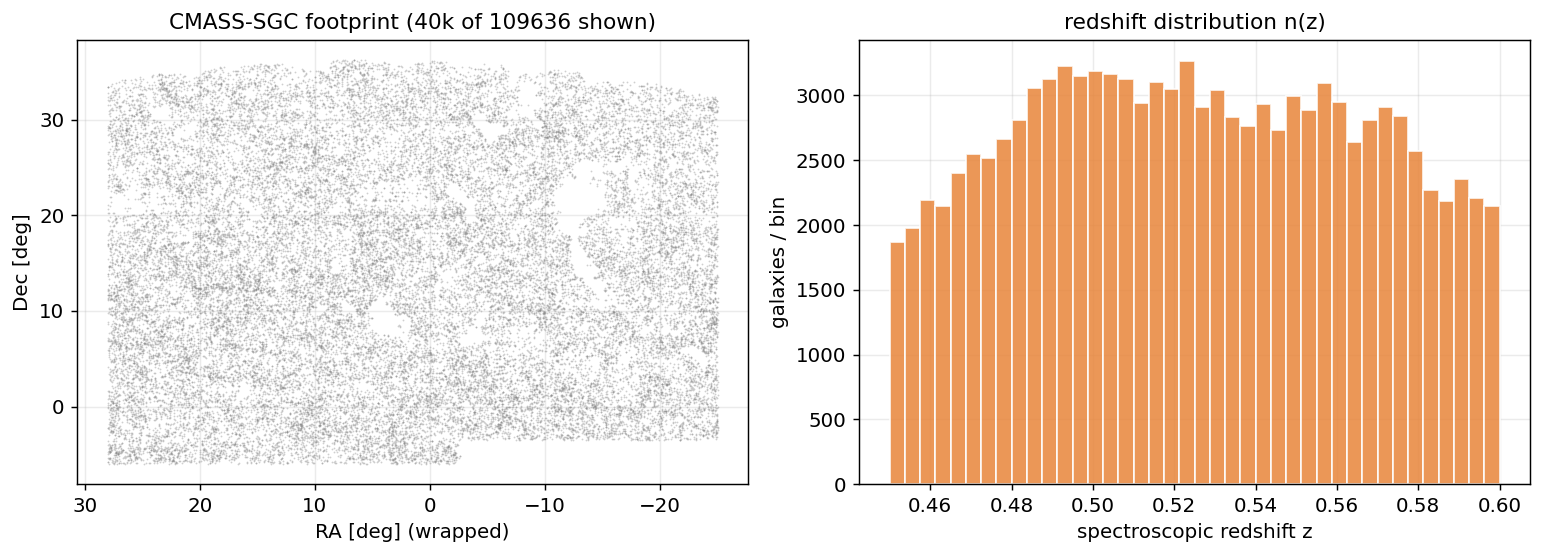
\includegraphics[width=0.49\textwidth]{footprint.png}
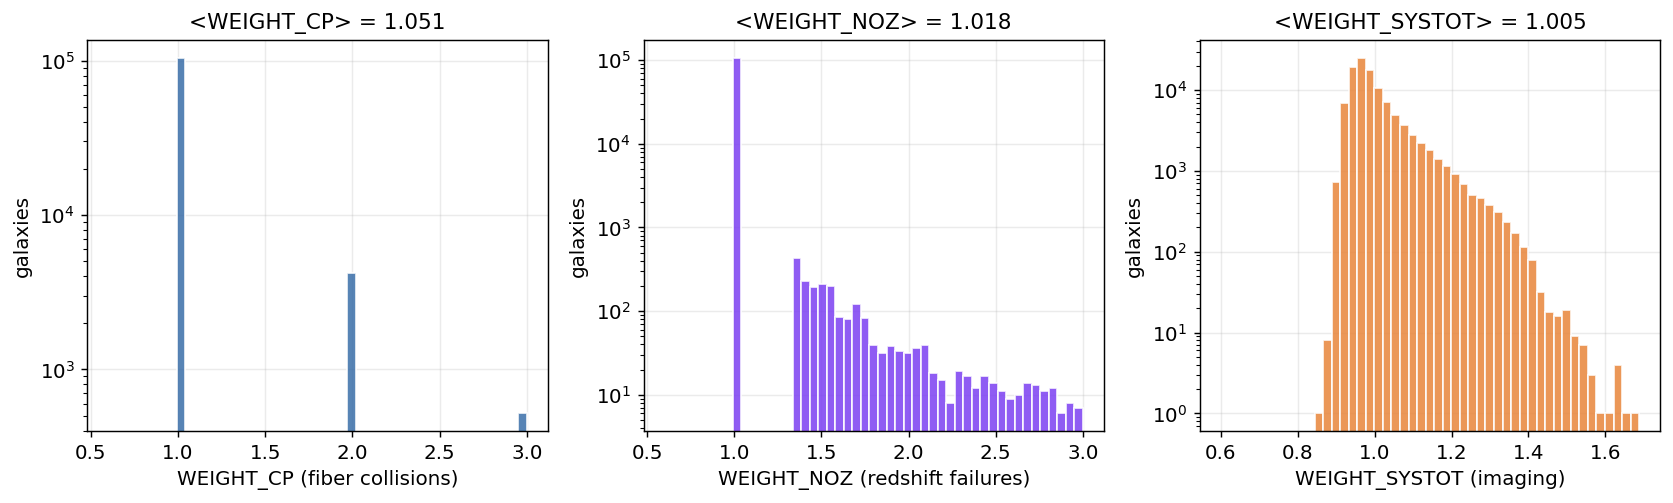
\includegraphics[width=0.49\textwidth]{weights.png}
\caption{BOSS CMASS-South geometry and completeness inputs.  The completion is
conditioned on the observed BOSS footprint, the published completeness weights,
and the SDSS imaging positions of spectroscopically missing targets.}
\label{fig:footprint_weights}
\end{figure*}

\begin{figure}
\centering
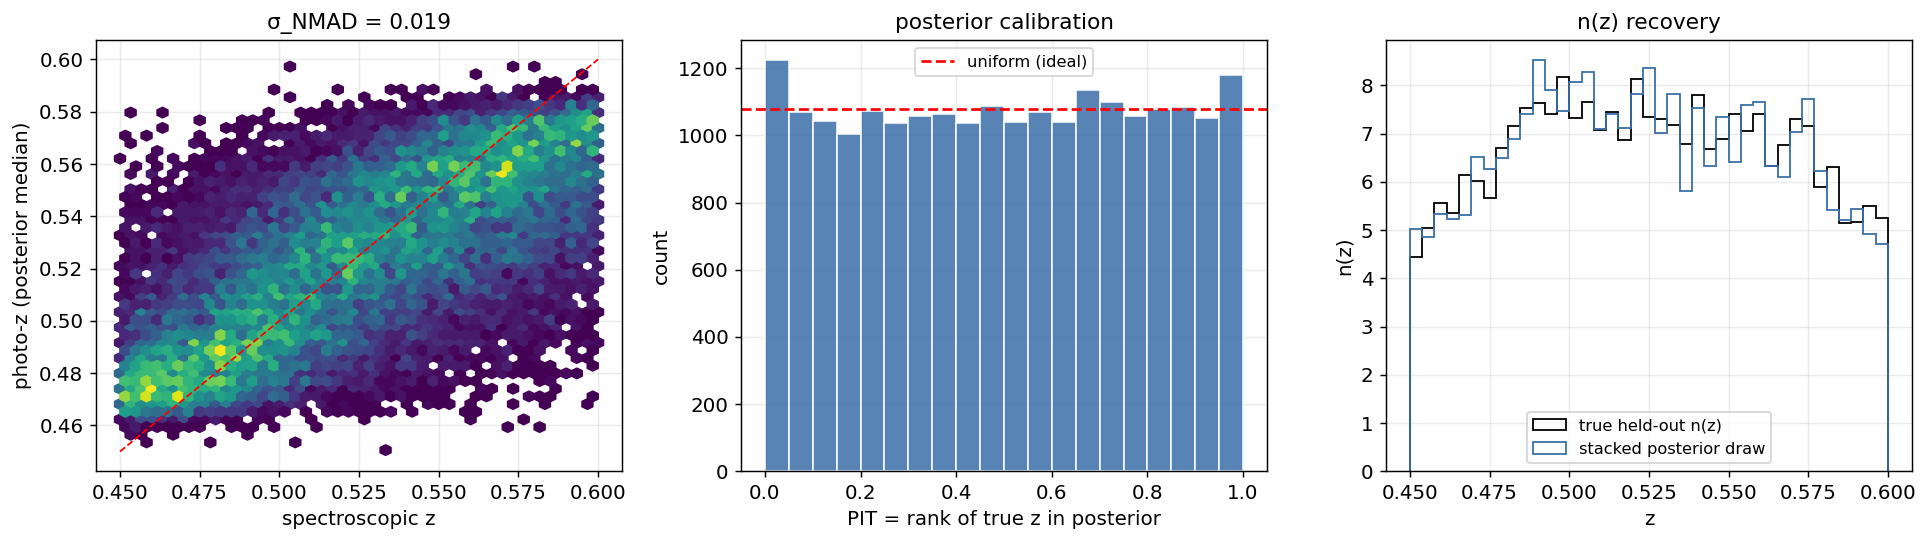
\includegraphics[width=\columnwidth]{photoz.png}
\caption{Color-space $k$NN photo-$z$ diagnostic for the CMASS sample.  The
photo-$z$ is used as a likelihood factor for missing redshifts, not as a
standalone redshift assignment.}
\label{fig:photoz}
\end{figure}

\subsection{Local-density redshift posterior}
\label{subsec:localdensity}

The default redshift engine is a fast local-density approximation to a
conditional field posterior.  For missing target $i$ at angular position
$\hat{\bf n}_i$ and colors ${\bf x}_i$, redshifts are sampled from
\begin{equation}
  p_i(z) \propto
  \widehat{\lambda}_{\rm loc}(\hat{\bf n}_i,z)\,
  \widehat{p}_{\rm col}(z\mid{\bf x}_i)\,
  q_i(z),
  \label{eq:localposterior}
\end{equation}
where $\widehat{p}_{\rm col}$ is the color-space photo-$z$ density, $q_i$ is an
empirical close-pair prior for collisions and unity for redshift failures, and
$\widehat{\lambda}_{\rm loc}$ is the observed local line-of-sight density.  The
local density is estimated from the $K=150$ nearest observed spectroscopic
galaxies in angular unit-vector space:
\begin{equation}
  \widehat{\lambda}_{\rm loc}(\hat{\bf n}_i,z) =
  \sum_{j\in{\cal N}_K(i)}
  \exp\left[-\frac{(z-z_j)^2}{2\sigma_f^2}\right],
  \qquad \sigma_f=0.004 .
\end{equation}
The photo-$z$ factor is evaluated on the same 256-point redshift grid with a
Gaussian smoothing scale $\sigma_p=0.02$ applied to the neighbor redshifts and
their $k$NN weights.  For collided targets, $q_i(z)$ is the symmetrized
histogram of redshift differences among observed close pairs within $62''$,
measured directly from the data over $|\Delta z|<0.06$.  The sampled redshift is
then jittered by a Gaussian of width $\sigma_f/2$ and clipped to the CMASS
redshift interval.

Equation (\ref{eq:localposterior}) is deliberately observational.  It does not
assign a missing galaxy to a simulated halo or require a fiducial cosmology.
The object is placed at its real angular position and on a redshift structure
seen in the neighboring spectroscopy, with the color likelihood preventing the
local-density prior from assigning obviously incompatible redshifts.

\subsection{Imaging-systematic analogs and provenance}
\label{subsec:systot}

The BOSS imaging-systematic correction \texttt{WEIGHT\_SYSTOT} is a smooth
density correction, not a statement that a particular nearby target failed to
receive a fiber.  We therefore do not convert it into exact duplicate galaxies.
For every observed or spectroscopically restored base object, the sampler adds
\begin{equation}
  n_{\rm extra} =
  \left\lfloor \max(w_{\rm systot}-1,0)+U \right\rfloor,
  \qquad U\sim{\cal U}(0,1),
\end{equation}
local analogs at the same source position with a $1''$ Gaussian angular jitter
and the same redshift.  This preserves resolved angular and three-dimensional
clustering while avoiding a zero-separation spike that would corrupt
nearest-neighbor or counts-in-cells statistics.  The default implementation
keeps all real detections; it restores density deficits implied by
$w_{\rm systot}>1$ rather than thinning observed galaxies in regions with
$w_{\rm systot}<1$.

Each output object carries a provenance code: 0 for observed spectroscopy,
1 for restored fiber-collision target, 2 for restored redshift failure, 3 for
imaging-systematic analog, 4 for rare host-redshift fallback, and 5 for optional
mask inpainting.  The provenance vector is central to reproducibility because
analysts can rerun a statistic on individual components or test sensitivity to
the imaging analog prescription.

\subsection{Compact posterior and sampling}
\label{subsec:compact}

The default posterior has a simple product structure once the observed data are
fixed.  The observed galaxies never change across realizations.  The missing
galaxy positions never change.  The redshift posterior for each missing galaxy,
Equation (\ref{eq:localposterior}), is also fixed after it is computed.  A
realization is only a draw from each per-object inverse CDF plus the stochastic
imaging analogs.

The release stores the posterior as a compressed \texttt{npz} file.  It contains
the observed redshifts, the base RA and Dec arrays for observed plus restored
targets, the base provenance vector, \texttt{WEIGHT\_SYSTOT}, and an inverse CDF
for each of the 6,777 missing targets.  The inverse CDF is tabulated at 65
quantile levels and quantized to \texttt{uint16}.  The file
\texttt{cmass\_south\_posterior.npz} is 2.04 MB.  A matching uniform-footprint
random catalog, \texttt{cmass\_south\_randoms.npz}, contains 438,544 points.
Because CMASS-South is approximately 99\% complete in the angular random mask,
these randoms are uniform over the footprint to the percent level.

Sampling is deterministic under a seed:
\begin{enumerate}
\item draw one uniform variate for each missing target and invert its stored
redshift CDF;
\item concatenate the fixed observed galaxies and the restored targets;
\item draw local analog counts from \texttt{WEIGHT\_SYSTOT};
\item return arrays \texttt{ra}, \texttt{dec}, \texttt{z}, \texttt{prov}, and
\texttt{N}.
\end{enumerate}
For seed 0, the sampled catalog contains 119,923 objects: 109,636 observed,
5,272 collision restorations, 1,505 redshift-failure restorations, and 3,510
smooth-systematic analogs.  Without the imaging analogs, the fixed base catalog
contains 116,413 objects.

\begin{figure*}
\centering
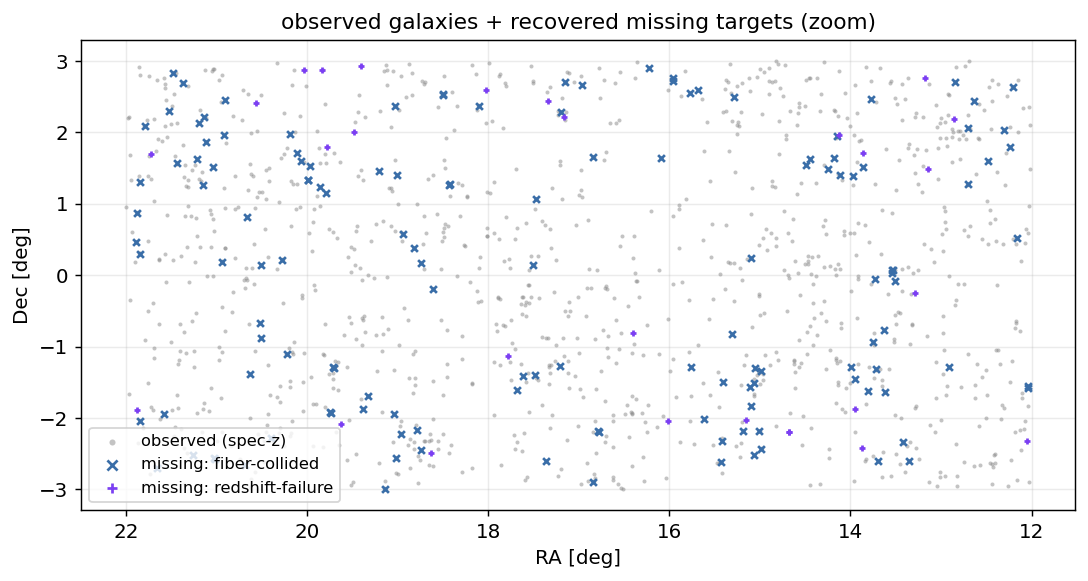
\includegraphics[width=0.49\textwidth]{missing.png}
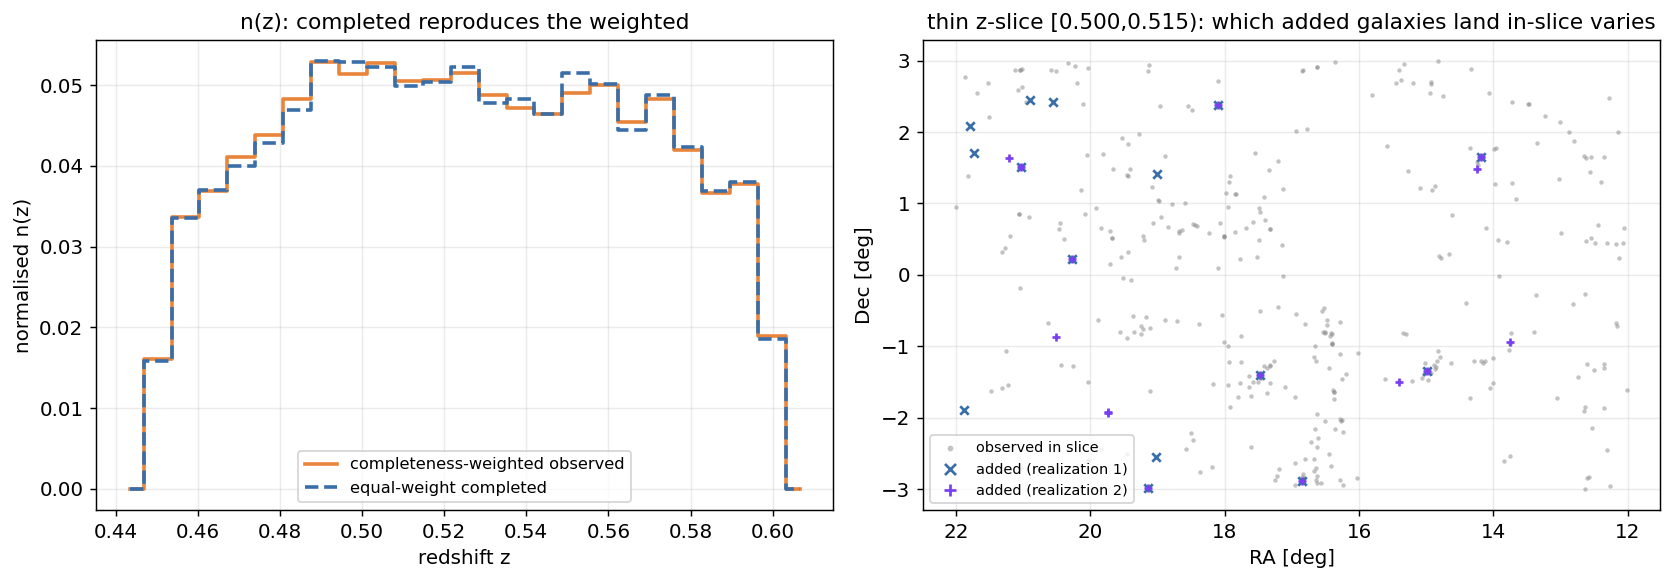
\includegraphics[width=0.49\textwidth]{samples_nz.png}
\caption{Missing-target recovery and sampled redshift distributions.  The
restored galaxies are placed at real imaging positions, and only their
redshifts are sampled.  Realizations differ in the redshifts of missing
galaxies and in the stochastic imaging-systematic analogs.}
\label{fig:missing_nz}
\end{figure*}

\subsection{Clustering measurements and acceptance metrics}
\label{subsec:metrics}

For angular clustering we measure Landy--Szalay estimates
\citep{LandySzalay1993} with the fixed random catalog.  For three-dimensional
statistics we use \texttt{Corrfunc} \citep{Corrfunc2020}.  The catalog itself is
cosmology-free; \texttt{Corrfunc} measurements convert redshift to comoving
distance at measurement time, using the analyst's fiducial cosmology, and then
call the OpenMP mock pair counters with \texttt{is\_comoving\_dist=True}.  The
main validation statistics are $w(\theta)$, $w_p(r_p)$, $\xi(r_p,\pi)$, and
redshift-space multipoles $\xi_0(s)$ and $\xi_2(s)$.  We also evaluate
higher-order or non-two-point summaries: nearest-neighbor CDFs and
counts-in-cells.  These are deliberately included because the purpose of the
catalog posterior is to support statistics beyond those for which BOSS weights
were optimized.

The acceptance criteria are empirical.  In truth-known tests, the completed
ensemble should recover the truth catalog to the percent level over the scales
where the input mocks themselves are faithful.  On the real data, the
equal-weight completed catalogs should reproduce the official
$w_c=\texttt{WEIGHT\_SYSTOT}\,(\texttt{WEIGHT\_CP}+\texttt{WEIGHT\_NOZ}-1)$
weighted BOSS clustering within the known scale of the correction.  The
completion posterior spread should be smaller than the sample-variance
covariance for BOSS CMASS-South, because it represents only uncertainty in
observational completion conditioned on the observed catalog.

\section{The graphGP Complement}
\label{sec:graphgp}

The local-density engine in Section \ref{subsec:localdensity} is fast and
compressible, but it treats the missing-galaxy redshift posteriors as
conditionally independent once the observed catalog is fixed.  The graphGP
route is a complementary, more explicit field-level model.  It assumes that the
complete galaxy overdensity field can be approximated by a Gaussian process
with covariance tied to the observed two-point function, and that the observed
galaxies are noisy samples of that field.

Let $\delta({\bf x})$ be the galaxy overdensity in a fiducial comoving
coordinate system.  The graphGP prior is
\begin{equation}
  \delta({\bf x}) \sim {\cal GP}\left[0,K_\xi(|{\bf x}-{\bf x}'|)\right],
  \label{eq:gpprior}
\end{equation}
where $K_\xi(r)$ is a tabulated covariance derived from a Landy--Szalay
measurement of the galaxy correlation function.  The likelihood is a Gaussian
approximation to an inhomogeneous Poisson process.  At observed galaxy
locations ${\bf x}_D$, the data vector is
\begin{equation}
  y_i = \bar n_i^{-1}-1,\qquad
  N_{ii}=\bar n_i^{-1},
\end{equation}
where $\bar n_i$ is the local mean density implied by the survey selection.
The posterior is Gaussian:
\begin{align}
  \mu_{\rm post}({\bf x}) &=
  K({\bf x},{\bf x}_D)\,[K_{DD}+N]^{-1}y_D,\\
  C_{\rm post}({\bf x},{\bf x}') &=
  K({\bf x},{\bf x}') -
  K({\bf x},{\bf x}_D)\,[K_{DD}+N]^{-1}K({\bf x}_D,{\bf x}').
\end{align}

The implementation samples this posterior by Matheron's rule
\citep{RybickiPress1992}.  A prior draw $\delta_{\rm prior}$ is generated on a
sparse neighbor graph using a Vecchia-style approximation
\citep{Katzfuss2020,Schafer2021}.  The conditional draw is
\begin{equation}
  \delta_{\rm post}({\bf x}) =
  \delta_{\rm prior}({\bf x})
  + K({\bf x},{\bf x}_D)[K_{DD}+N]^{-1}
  \left[y_D-\delta_{\rm prior}({\bf x}_D)\right].
  \label{eq:matheron}
\end{equation}
The expensive solve is amortized over many missing-galaxy redshift draws.  The
primary stored object is a light-cone-native array
$1+\delta_{\rm post}$ on redshift shells and HealPIX pixels.  For a missing
galaxy, graphGP replaces the local KDE in Equation (\ref{eq:localposterior}) by
the corresponding field draw:
\begin{equation}
  p_i(z\mid s) \propto
  [1+\delta_{\rm post}^{(s)}(\hat{\bf n}_i,z)]\,\bar n(z)\,
  \widehat{p}_{\rm col}(z\mid{\bf x}_i)\,q_i(z).
  \label{eq:graphgpz}
\end{equation}
All missing galaxies in realization $s$ share the same density-field draw, so
their redshift assignments are correlated.

This model has a fiducial comoving coordinate system internally because a
three-dimensional covariance needs a distance.  That coordinate system is a
modeling gauge for the field interpolation, not a cosmology baked into the
released KNN product.  The report tests this explicitly by rebuilding the
graphGP route with different fiducial distance-redshift relations.  Planck-like
and Einstein--de Sitter choices give per-object redshift RMS differences of
about 0.001--0.0012, correlations of 0.9995--0.9996, and changes in
$w_p(r_p)$ below 0.1\%.  Within the accuracy demanded by the present BOSS
completion, graphGP is therefore best viewed as a correlated posterior engine
whose output is stable to reasonable internal coordinate choices.

\section{Application to BOSS DR12 CMASS-South}
\label{sec:application}

\subsection{Why BOSS is the right test case}
\label{subsec:boss_context}

BOSS DR12 is the ideal laboratory because the official two-point analyses are
mature.  The survey, target selection, and LSS catalogs are documented
\citep{Dawson2013,Reid2016}, the spectroscopic system is understood
\citep{Smee2013}, the DR12 cosmology and systematic-correction papers provide
community reference measurements \citep{Alam2017,Ross2017}, and independent
mock suites such as MultiDark-Patchy exist for validation
\citep{Kitaura2016}.  A completed-catalog product can therefore be judged
against a well-established reference: it should reproduce the weighted BOSS
two-point measurements while exposing a point catalog suitable for statistics
that were not part of the official BOSS pipeline.

The official BOSS correction strategy keeps the observed spectroscopic catalog
and supplies per-object weights.  Close-pair and redshift-failure weights move
the missing object's statistical weight to an observed neighbor, while
\texttt{WEIGHT\_SYSTOT} corrects smooth density modulations associated with
imaging and observing conditions.  Random catalogs encode the angular mask and
radial selection.  This system is extremely effective for the published
two-point program, but for a general statistic the analyst must decide how to
apply weights, whether the statistic is linear or nonlinear in those weights,
and how random catalogs should enter.
Fiber-collision corrections illustrate the point: nearest-neighbor upweighting
and more refined pairwise or angular correction schemes can be calibrated for
two-point functions \citep{Guo2012,Mohammad2020}, but they do not automatically
define how a nonlinear statistic should respond to a missing close pair.

SIMBIG is a useful modern comparison point.  It uses BOSS CMASS-South-like cuts
and a forward-modeling program to connect nonlinear galaxy clustering
statistics to cosmological parameters \citep{Hahn2023Mock,Hahn2023PNAS,
Hahn2024NatAs,Hahn2024Bispectrum}.  Later work extends the same style of
analysis to summaries such as the wavelet scattering transform and marked power
spectra \citep{Regaldo2024,Massara2025SBI}.  The scientific ambition is close
to ours--to use information beyond the Gaussian two-point limit--but the
observational interface remains the published BOSS selection and weighting
system.  Our product is complementary: it provides an ensemble of completed
data catalogs so the observational correction can be sampled once and then
reused by any statistic.

\subsection{Default KNN-field completion}
\label{subsec:boss_default}

The default BOSS ECHOES product uses the KNN-field engine.  The report's top-level
numbers are as follows.  The observed catalog has 109,636 CMASS-South galaxies.
The real missing-target list contains 5,272 collision targets and 1,505
redshift-failure targets.  The fixed base catalog therefore has 116,413
galaxies.  With the imaging-systematic analog sampler enabled, seed 0 has
119,923 galaxies, including 3,510 analogs.  Seeds 0--4 vary only at the
$\simeq 0.1\%$ level in total count, as expected for the smooth analog step.

Figure \ref{fig:missing_nz} shows the restored-target population and sampled
$n(z)$.  Figure \ref{fig:twopoint} compares angular and two-dimensional
clustering.  The completed equal-weight catalogs reproduce the official
weighted angular clustering to roughly 1.5\% over the plotted angular range and
the projected and multipole statistics at the 1--5\% level, depending on scale
and statistic.  This is the expected accuracy target: the completed catalog is
not an exact algebraic rewrite of the official weights, because it assigns
redshifts and positions to missing galaxies rather than moving all their weight
onto observed neighbors, but it should remain inside the systematic scale
already tolerated by the reference BOSS treatment.

\begin{figure*}
\centering
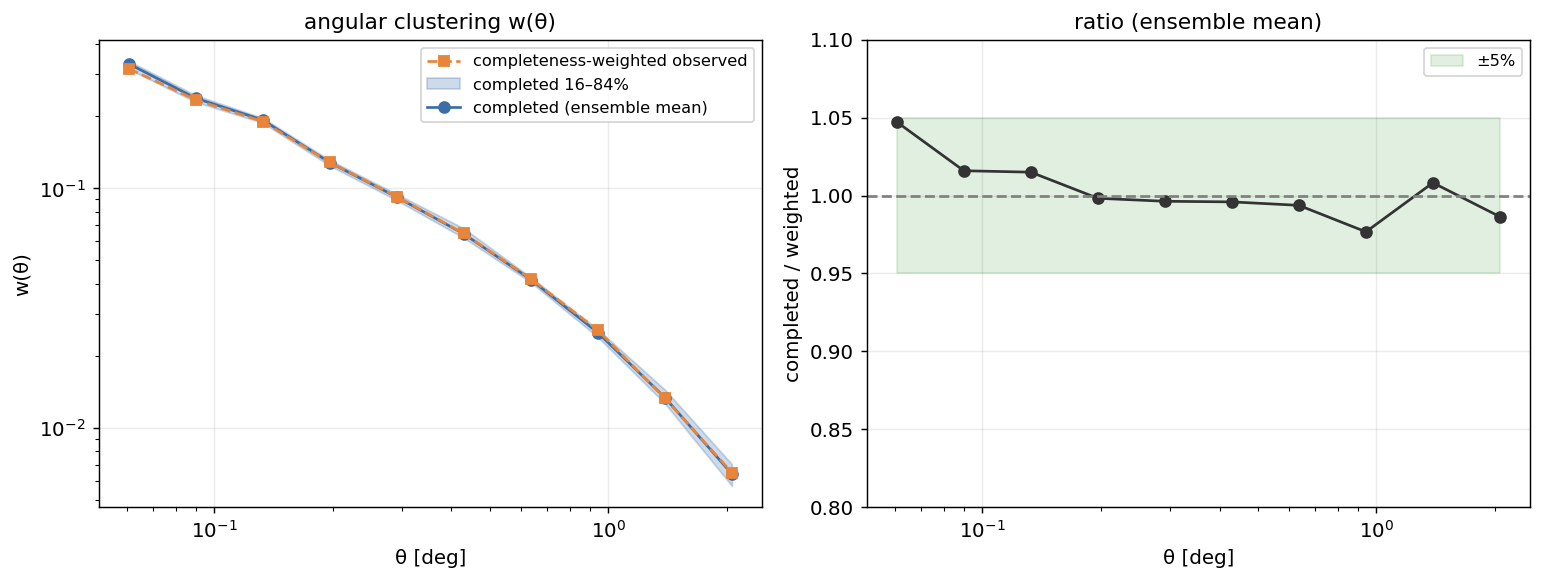
\includegraphics[width=0.49\textwidth]{wtheta.png}
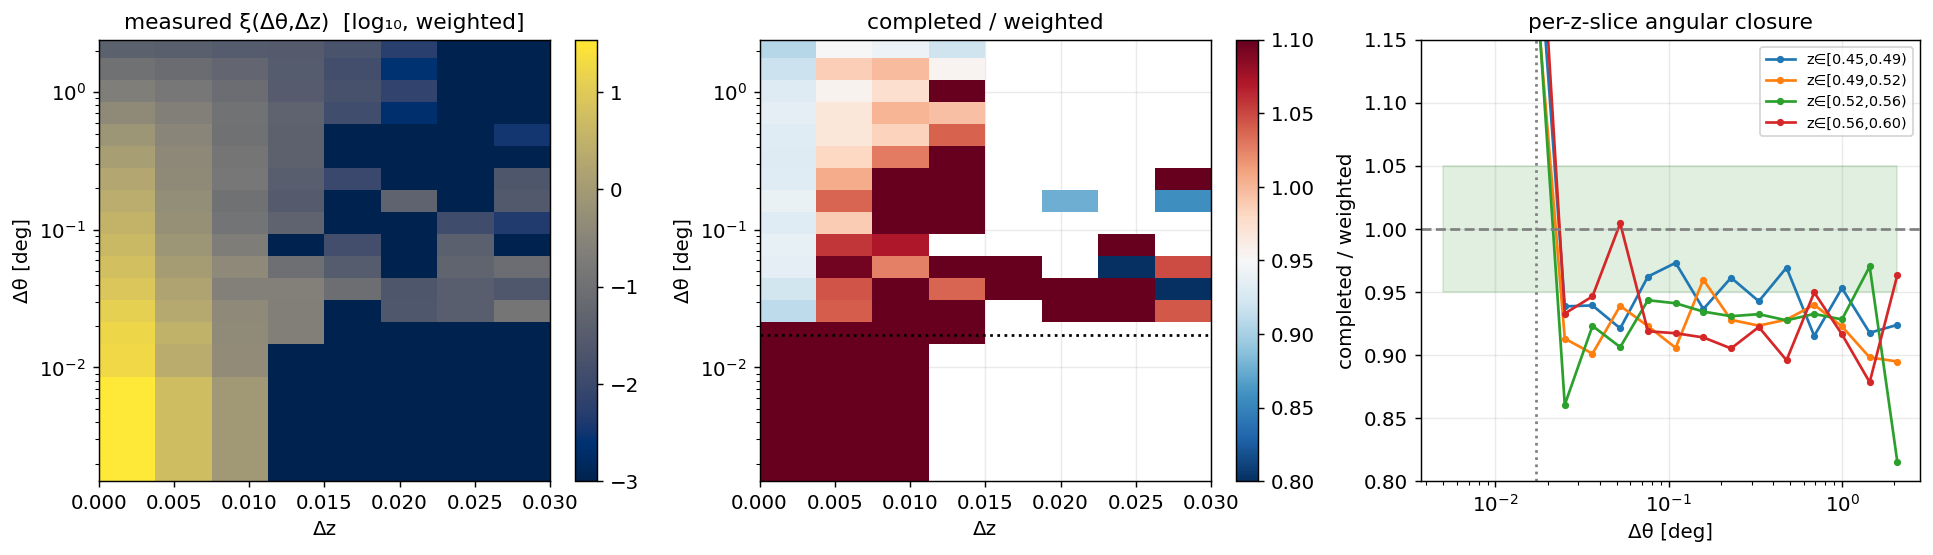
\includegraphics[width=0.49\textwidth]{xi2d.png}
\caption{Two-point validation on the real BOSS CMASS-South data.  The
equal-weight completed catalogs reproduce the official weighted angular and
redshift-space clustering while replacing completeness weights by explicit
galaxies.}
\label{fig:twopoint}
\end{figure*}

\subsection{Truth-known validation}
\label{subsec:truth}

Two truth-known tests are used.  The first hides the spectroscopic redshifts of
a subset of real BOSS galaxies and then asks the completion machinery to recover
the clustering of the original full catalog.  The second applies the same
machinery to independent MultiDark-Patchy mocks.  In both tests, an ``oracle''
catalog that restores the hidden objects with their true redshifts provides a
floor: if the oracle differs from truth, the difference comes from the masking
and bookkeeping rather than from redshift assignment.

The main result is shown in Figure \ref{fig:truth}.  The real-BOSS-truth mock
and the Patchy mocks recover $w_p(r_p)$ to about 1--2\% over
$0.5<r_p<40\,h^{-1}{\rm Mpc}$.  The oracle ratio lies in the range
0.997--1.005, so the remaining error is dominated by the redshift assignment
posterior.  The Patchy test is faithful above about
$1\,h^{-1}{\rm Mpc}$; the sub-Mpc deficit is a known one-halo limitation of the
Patchy mocks rather than a failure mode inferred from real BOSS data.

\begin{figure*}
\centering
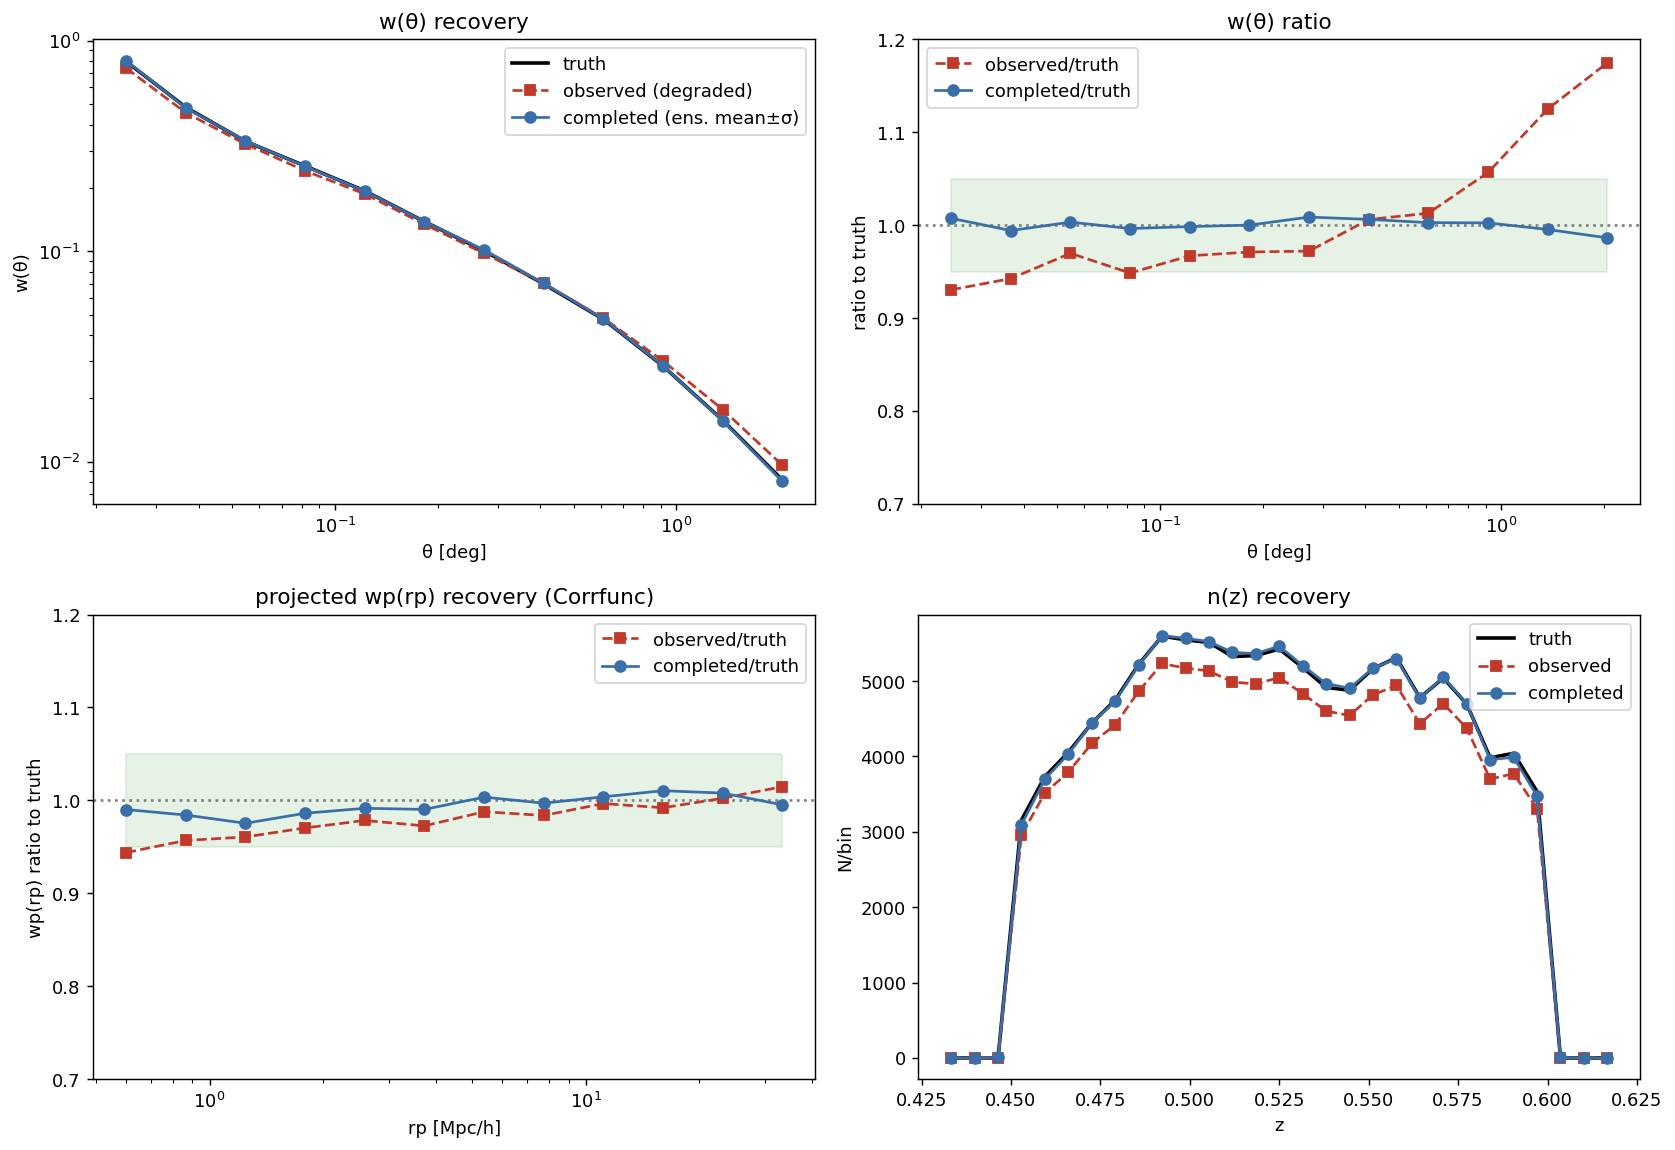
\includegraphics[width=0.49\textwidth]{mock_truth_recovery.png}
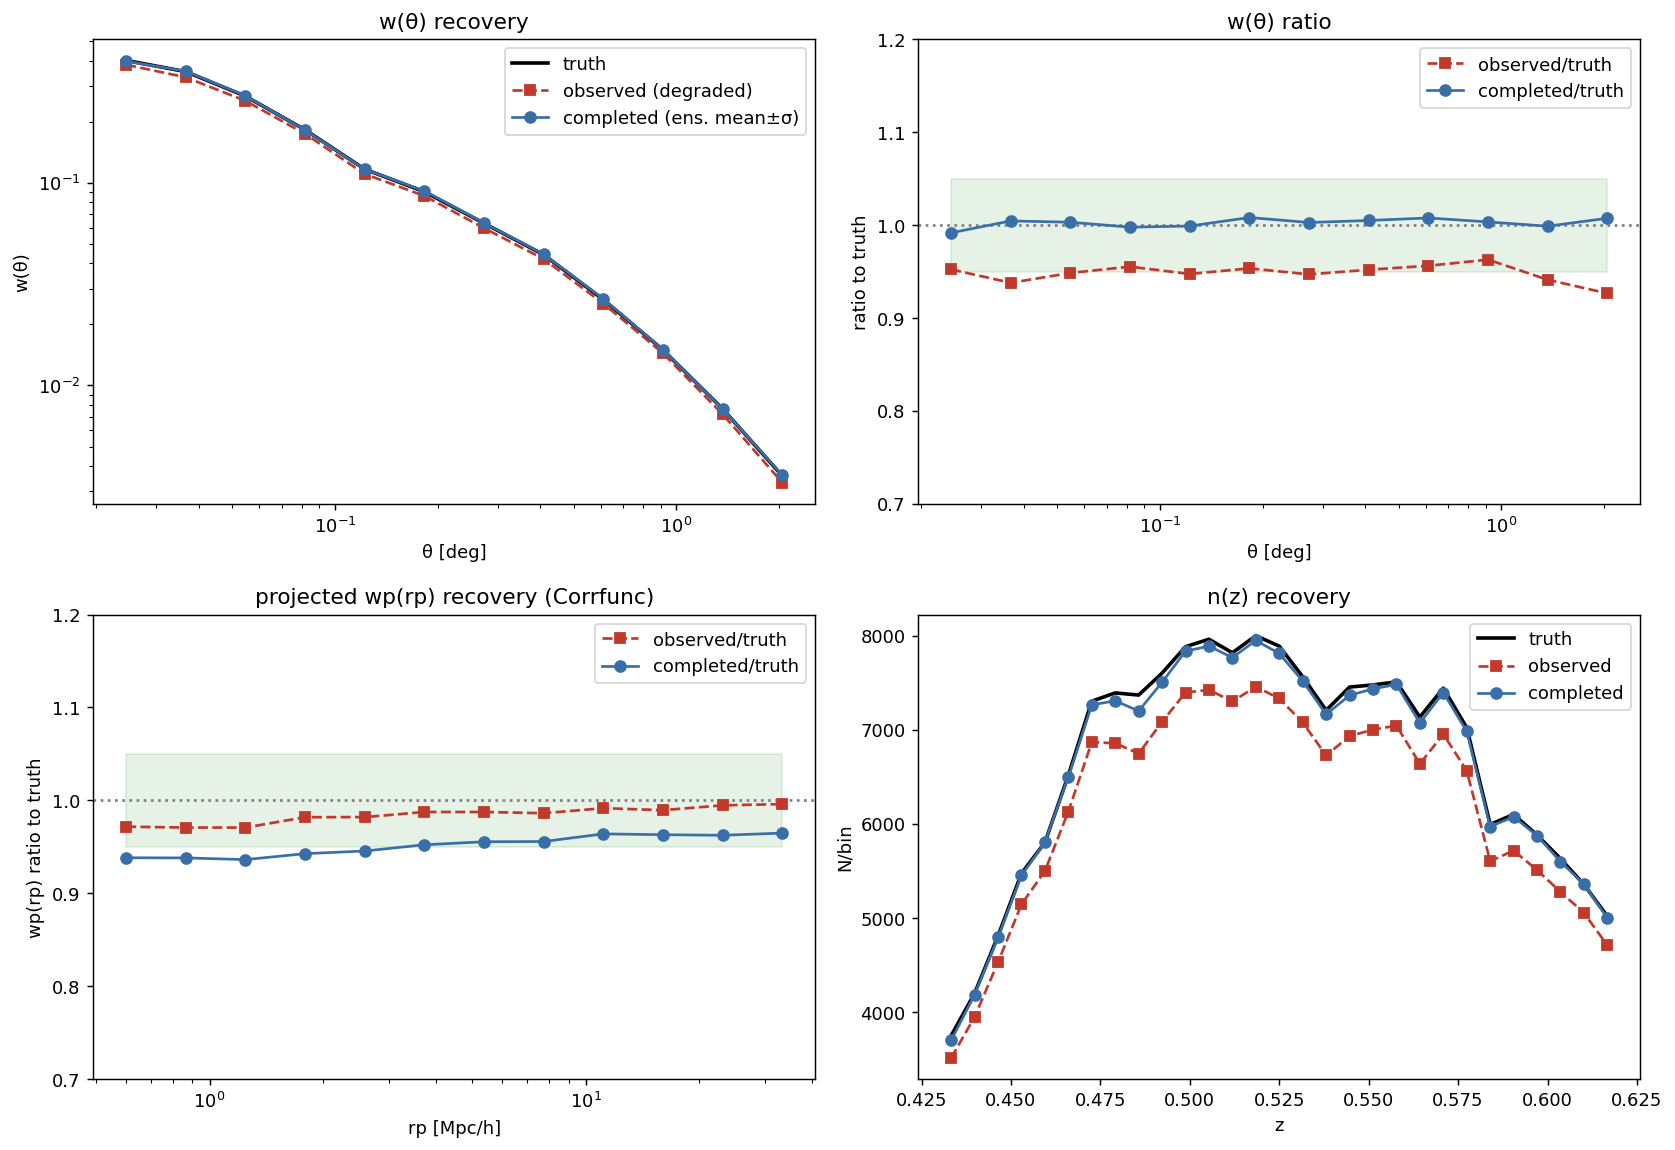
\includegraphics[width=0.49\textwidth]{patchy_truth_recovery.png}
\caption{Truth-known recovery tests.  The completed ensemble recovers the input
projected clustering at the 1--2\% level over the validated scales.  The oracle
curve isolates the part of the residual that comes from redshift assignment.}
\label{fig:truth}
\end{figure*}

\subsection{Higher-order and non-two-point checks}
\label{subsec:higherorder}

The validation intentionally includes summaries that are nonlinear in the point
set.  For nearest-neighbor CDFs, the maximum absolute CDF differences between
completed and truth catalogs are 0.0022, 0.0021, and 0.0011 for $k=1,2,4$,
respectively.  For counts in $8\,h^{-1}{\rm Mpc}$ cells, the mean is 0.660
versus 0.663 in truth, the variance-to-mean ratio is 2.37 versus 2.42, and the
skewness is 2.90 versus 2.94.  These tests are not exhaustive, but they are
important because a product that only reproduces $w_p$ could still fail for
nearest-neighbor or cell-count statistics.

\begin{figure}
\centering
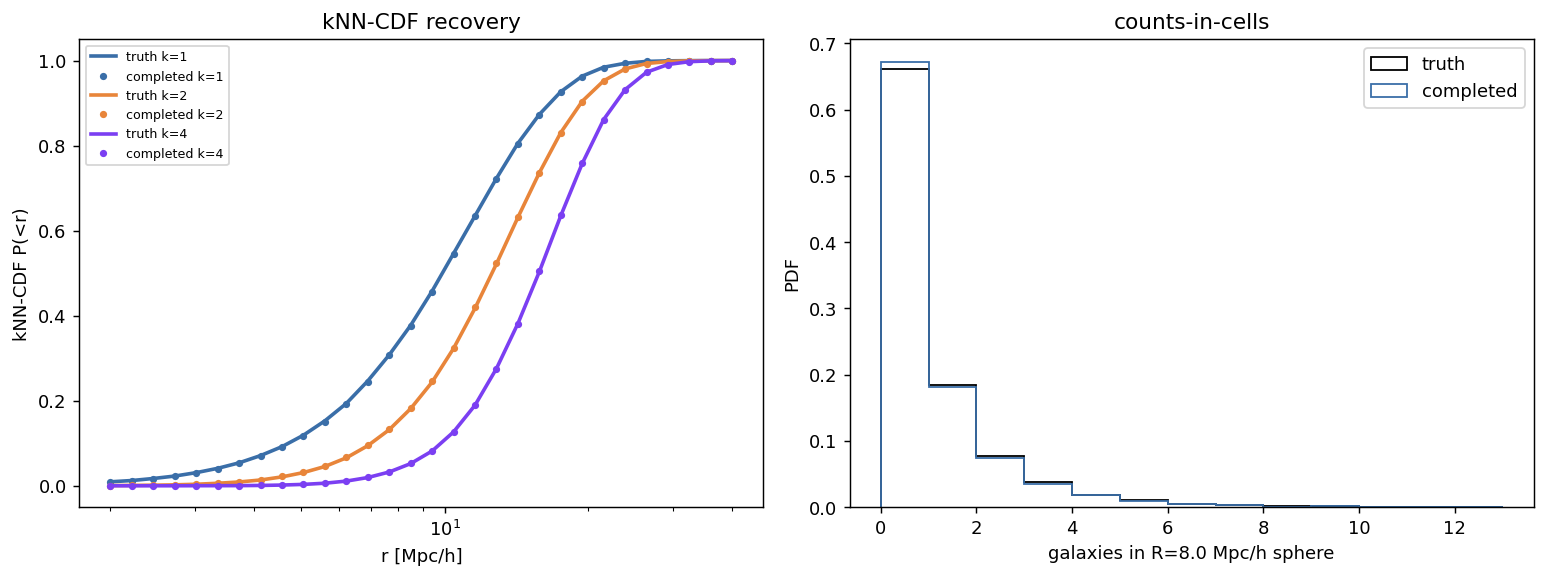
\includegraphics[width=\columnwidth]{completion_highorder.png}
\caption{Higher-order validation with nearest-neighbor CDFs and
counts-in-cells.  These diagnostics probe nonlinear responses to duplicate
points, missing close pairs, and redshift smearing.}
\label{fig:highorder}
\end{figure}

\subsection{Calibration of completion uncertainty}
\label{subsec:calibration}

The completion posterior is intentionally narrower than a full survey
posterior.  It conditions on the observed CMASS-South realization and resamples
only the unobserved spectroscopic information and smooth imaging analogs.  In
the Patchy calibration suite, the posterior uncertainty in $w_p(r_p)$ is
0.17--0.44\% per bin, while sample variance over the same bins is 0.8--7.2\%.
The completion therefore adds only 6--36\% of the sample-variance error in
quadrature, depending on scale.  The 68\% completion band brackets the mock
truth in only about 8\% of bins because it is not intended to regenerate the
large-scale density field.  This is correct behavior: a user should add the
completion covariance to a cosmic-variance or simulation covariance, not
replace that covariance with the completion ensemble.

\begin{figure}
\centering
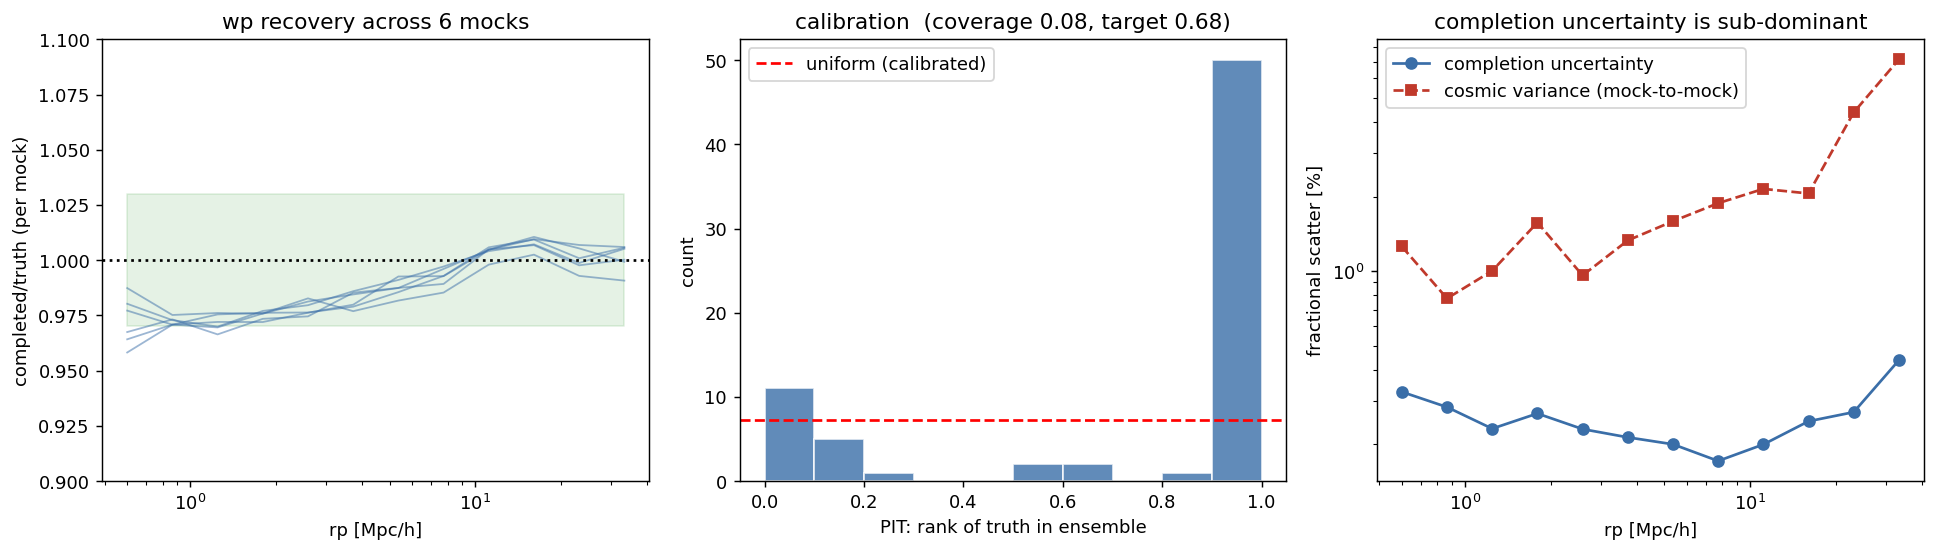
\includegraphics[width=\columnwidth]{recovery_calibration.png}
\caption{Calibration of the completion uncertainty relative to mock
sample variance.  The ensemble spread is the uncertainty in the observational
completion conditioned on the observed catalog, not the total survey
covariance.}
\label{fig:calibration}
\end{figure}

\subsection{KNN-field versus graphGP}
\label{subsec:graphgp_results}

The KNN-field and graphGP routes agree on the main scientific conclusion but
make different compromises.  The KNN-field engine is sharper on the sub-Mpc
collision scale because it directly uses nearby observed redshifts and the
empirical close-pair prior.  graphGP is smoother and more explicitly correlated
across missing objects because all lines of sight share a density-field draw.
In truth recovery, both routes recover the input clustering to the percent
level.  In the real-data head-to-head comparison, graphGP lies closer to the
official weighted reference on larger projected scales, with a typical ratio
near unity, while the KNN-field realization is modestly high in some bins.
Because the KNN-field route is much cheaper and compresses to the 2 MB public
ECHOES posterior, it is the default release.  graphGP is retained as a first-class
alternative for surveys or statistics where correlated redshift-completion
uncertainty is essential.

\begin{figure*}
\centering
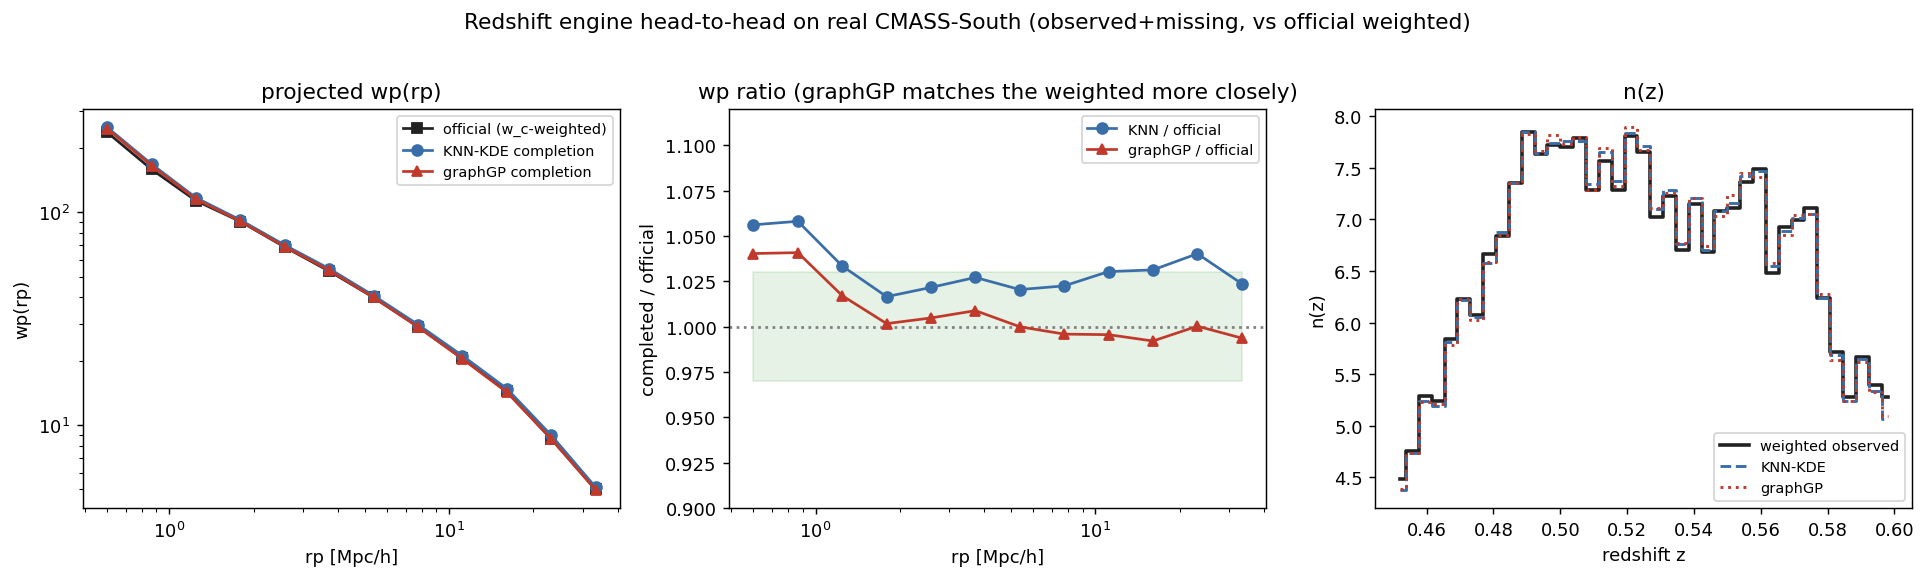
\includegraphics[width=0.49\textwidth]{graphgp_vs_knn.png}
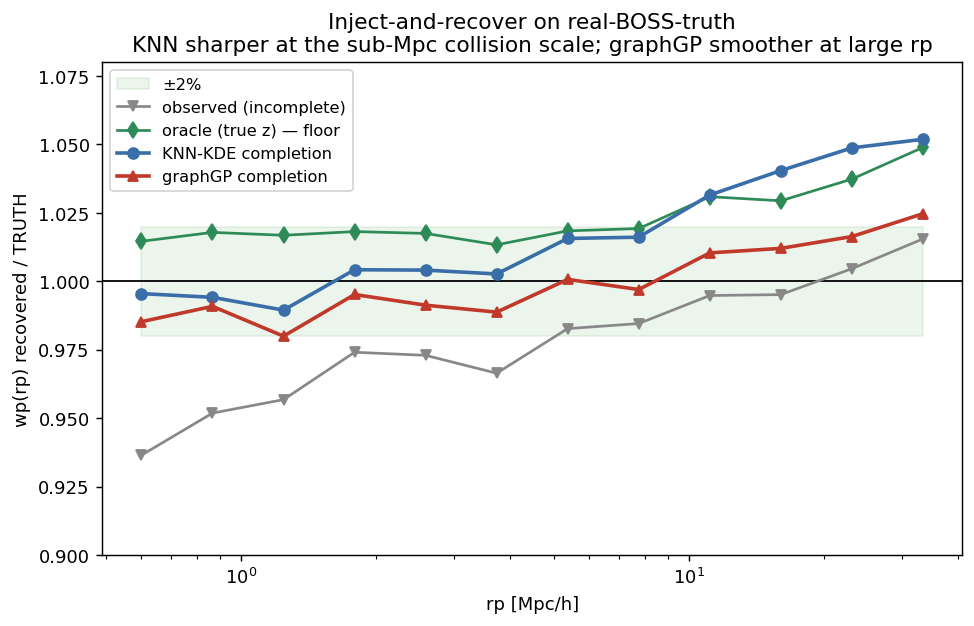
\includegraphics[width=0.49\textwidth]{graphgp_truth_recovery.png}
\caption{Comparison of the default KNN-field redshift engine with the
graphGP conditional-field route.  The two methods are complementary:
KNN-field is fast and local; graphGP is correlated through a shared posterior
density-field draw.}
\label{fig:graphgp}
\end{figure*}

\section{Sampling the Completion Posterior}
\label{sec:posterior}

For the default ECHOES release, a posterior sample is a completed catalog seed.  The
mean of a statistic over seeds estimates the statistic for the completed
survey, and the covariance over seeds estimates uncertainty due to the
completion.  If $S[{\cal C}^{(s)}]$ is any statistic of a catalog, then
\begin{align}
  \bar S &= \frac{1}{N_s}\sum_{s=1}^{N_s} S[{\cal C}^{(s)}],\\
  C_{ab}^{\rm comp} &=
  \frac{1}{N_s-1}\sum_s
  \left(S_a[{\cal C}^{(s)}]-\bar S_a\right)
  \left(S_b[{\cal C}^{(s)}]-\bar S_b\right).
\end{align}
This covariance should be added to, or modeled jointly with, the ordinary
survey covariance.  It should not be interpreted as the covariance of the
cosmological density field.

For graphGP the same equations apply, but the meaning of a seed changes.  A
seed selects a conditional density-field draw as well as the missing-galaxy
redshift draws from Equation (\ref{eq:graphgpz}).  The redshift assignments are
therefore correlated across missing galaxies.  This is the more faithful
posterior object if the statistic is sensitive to coherent redshift
uncertainty, but it is more expensive to construct and store.  For the BOSS
CMASS-South tests in this paper, the difference between graphGP and KNN-field
is smaller than the sample-variance error budget for the standard clustering
statistics.

The report evaluates several statistic-level responses.  The angular
$w(\theta)$ response to shifting the missing-galaxy redshift prior is far below
the realization scatter, as expected for a mostly angular statistic.  Radial
statistics are more sensitive.  The completed $w_p(r_p)$ correction uncertainty
is at the 0.2--0.4\% level, and the real-data comparison with official
weighted BOSS clustering is at the 1--5\% level across the displayed projected
and multipole statistics.  For nonlinear summaries, the nearest-neighbor CDF
and counts-in-cells tests in Figure \ref{fig:highorder} show no large hidden
failure from the local analogs or from the missing-redshift posterior.  Users
can repeat the same exercise for any proposed summary by running that summary
on seeds $0,\ldots,N_s-1$.

\section{Systematics, Masks, and Trustworthiness}
\label{sec:systematics}

The completion also produces diagnostic maps rather than only final catalogs.
The redshift-failure coupling to the local target density is consistent with
zero in the current BOSS CMASS-South product, $h=-0.06\pm0.06$, while the
fiber-collision coupling is detected, $h=-0.24\pm0.03$.  This is physically
reasonable: collisions occur in denser angular environments.  The completed
density map correlates with the total-target density at 0.98, and the
trustworthiness map has a median scatter of 0.13.  These diagnostics identify
where the completion is extrapolating most strongly.

The optional mask-inpainting product fills 542 interior holes totaling
16.6 deg$^2$, about 0.9\% of the footprint.  The inpainting closure test is
approximately 1\% over $0.06^\circ$--$2^\circ$.  We keep this step optional
because different analyses may prefer to leave bright-star holes and small mask
features explicit in the random catalog.  The default product therefore
corrects spectroscopic incompleteness and smooth imaging weights while leaving
the official footprint visible.

\begin{figure*}
\centering
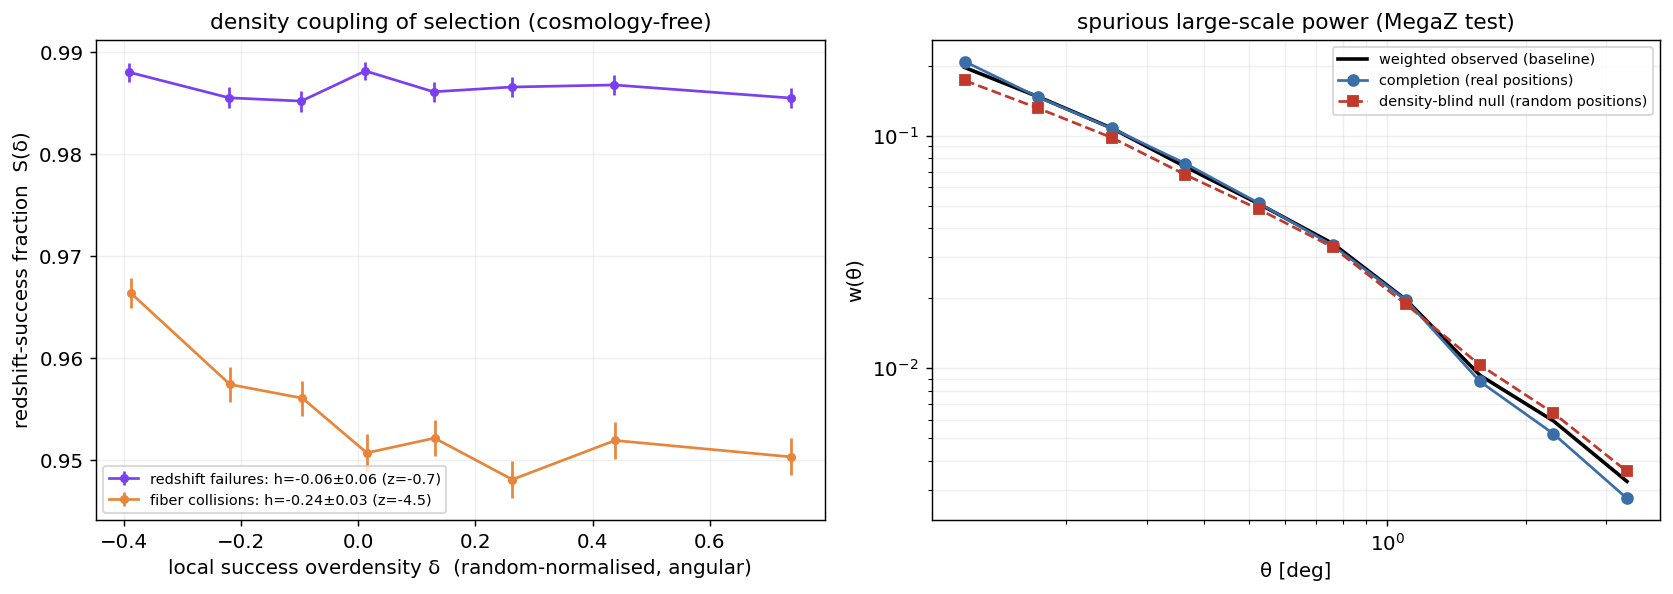
\includegraphics[width=0.32\textwidth]{coupling.png}
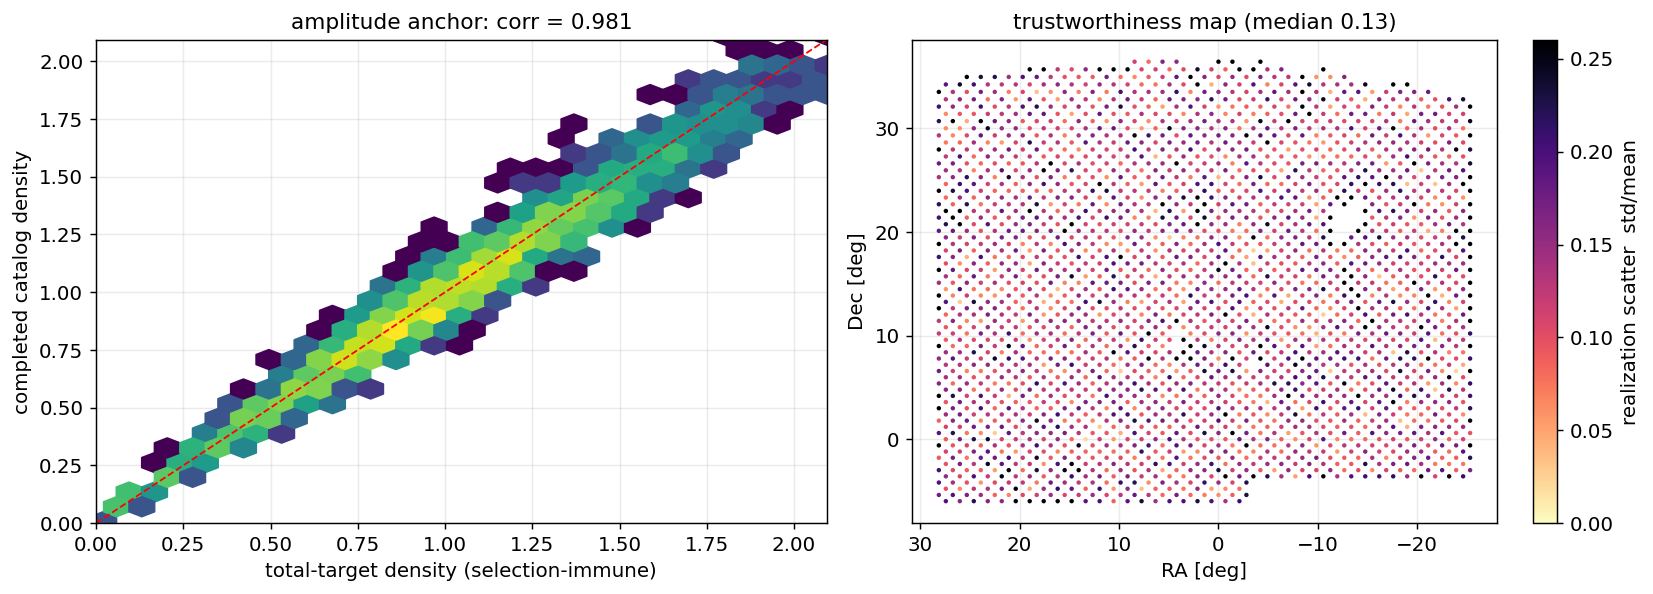
\includegraphics[width=0.32\textwidth]{trust.png}
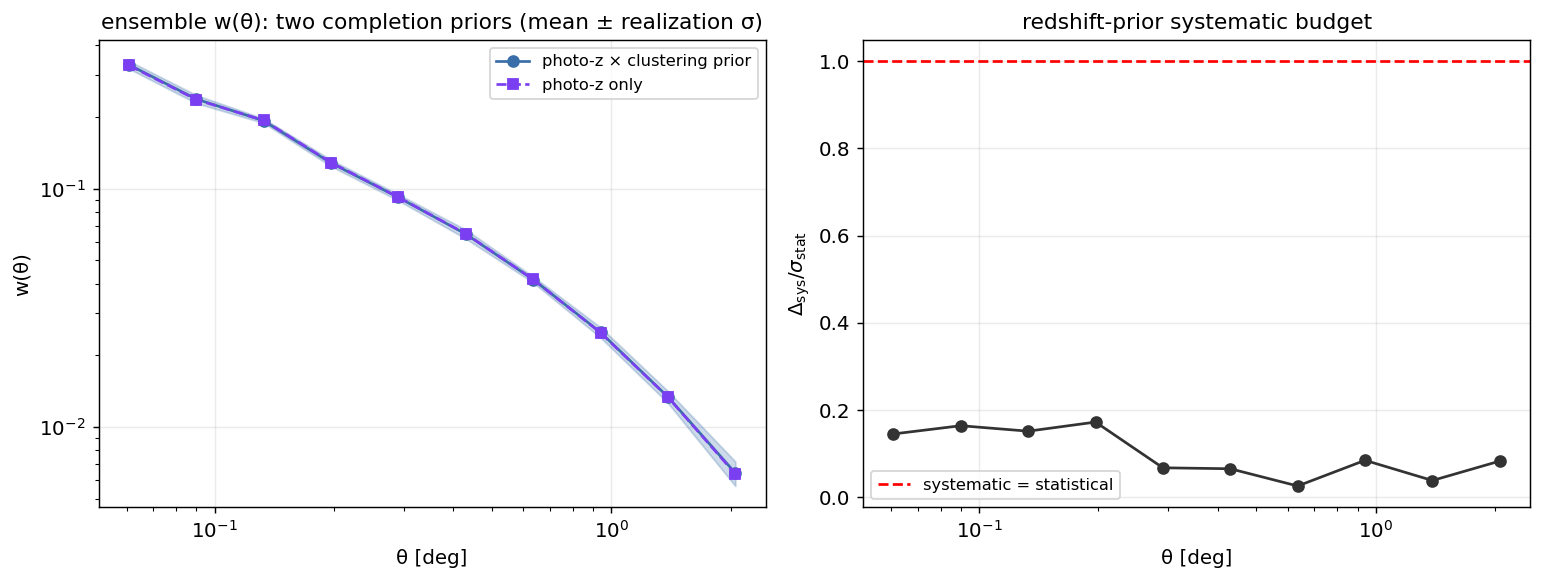
\includegraphics[width=0.32\textwidth]{systematics.png}
\caption{Systematics diagnostics for the completion.  The maps and coupling
tests quantify where the data-driven completion is well anchored by observed
targets and where it is most dependent on the model.}
\label{fig:systematics}
\end{figure*}

\section{Data and Code Availability}
\label{sec:availability}

The analysis code and ECHOES report products are in the public repository
\url{https://github.com/yipihey/graphGP-cosmology}.  The BOSS completion report
used for this manuscript is
\url{https://yipihey.github.io/graphGP-cosmology/completion.html}.  The compact
posterior and sampler are distributed in the report's \texttt{docs/data/}
directory:
\begin{verbatim}
cmass_south_posterior.npz
cmass_south_randoms.npz
draw_samples.py
\end{verbatim}
The minimal use pattern is
\begin{verbatim}
from draw_samples import load_package, draw
pkg = load_package("cmass_south_posterior.npz")
cat = draw(pkg, seed=0)
\end{verbatim}
which returns arrays \texttt{ra}, \texttt{dec}, \texttt{z}, \texttt{prov}, and
\texttt{N}.  A reproducible ensemble is specified by the integer seeds used.

The relevant source modules are \texttt{twopt\_density/boss.py} for the BOSS
loader, \texttt{twopt\_density/cmass\_targets.py} for missing target recovery,
\texttt{twopt\_density/photoz.py} for the color-space $k$NN photo-$z$,
\texttt{twopt\_density/observed\_ls.py} for the KNN-field completion and
graphGP redshift interface, \texttt{twopt\_density/posterior\_sampler.py} for
the compact inverse-CDF posterior, \texttt{twopt\_density/density\_field.py}
for graphGP posterior field sampling, and
\texttt{twopt\_density/clustering\_corrfunc.py} for the standard projected and
multipole clustering measurements.

\section{Conclusions}
\label{sec:conclusions}

We have presented \textsc{ECHOES}, an equal-weight completed-catalog posterior
for BOSS DR12 CMASS-South.  The product restores spectroscopically missing
galaxies at real SDSS imaging positions, samples their redshifts from a
data-driven posterior, and represents smooth imaging-systematic weights as
local analog galaxies.  It
therefore changes the user-facing data interface: instead of asking every new
summary statistic to understand the BOSS completeness weights, an analyst can
run the statistic directly on completed point catalogs and propagate
observational-completion uncertainty by resampling seeds.

The validation is deliberately conservative.  The completed ensemble recovers
truth-known $w_p(r_p)$ to the 1--2\% level over the validated scales, matches
official weighted BOSS clustering at the few-percent level, reproduces
nearest-neighbor CDFs and counts-in-cells diagnostics, and has a completion
uncertainty smaller than the CMASS-South sample variance.  The graphGP route
provides an independent, correlated posterior construction and agrees with the
default KNN-field route within the current BOSS error budget.

The broader implication is practical.  Survey collaborations have learned how
to publish two-point-ready data products.  The next generation of analyses will
not be limited to two-point functions, and the next generation of surveys will
have more complicated assignment, calibration, and selection functions.  A
ECHOES posterior over completed survey catalogs is a way to preserve the historical
division of labor--survey teams ground observational corrections in the data,
theory teams test statistics and models--while making the interface useful for
arbitrary summaries.  DESI, Euclid, Roman, CSST, and Rubin/LSST will all face
versions of this problem.  BOSS CMASS-South is small enough to solve carefully
and mature enough to validate against the standard answer; it is therefore a
useful prototype for how future public survey products can serve both standard
and beyond-two-point cosmology.

\appendix

\section{Reproducible Algorithm}
\label{app:algorithm}

This appendix writes the default KNN-field completion as an implementation
recipe.

\begin{enumerate}
\item Load the BOSS DR12 CMASS-South LSS catalog with photometry and the matching
random catalog.  Apply the cuts ${\rm RA}<28^\circ$ or ${\rm RA}>335^\circ$,
${\rm Dec}>-6^\circ$, and $0.45<z<0.60$.
\item Convert SDSS \texttt{MODELFLUX} and \texttt{EXTINCTION} to magnitudes and
colors.  Train \texttt{PhotoZKNN(k=100)} on finite observed galaxies using
features $(g-r,r-i,i-z,i)$.
\item Load the CMASS target catalog.  Build the missing list by greedily tying
no-spectrum targets to \texttt{WEIGHT\_CP} hosts within $62''$ and
\texttt{ZWARNING}$\ne0$ targets to \texttt{WEIGHT\_NOZ} hosts within $15'$.
\item Measure the observed close-pair $\Delta z$ pool from pairs of observed
galaxies within $62''$ and symmetrize it.
\item For each missing target, find the $K=150$ angular nearest observed
spectroscopic galaxies.  On a 256-point redshift grid, form the product of the
local field KDE with $\sigma_f=0.004$, the photo-$z$ KDE with
$\sigma_p=0.02$, and, for collisions, the close-pair prior.
\item Store each normalized posterior as a 65-level inverse CDF.  Quantize the
observed redshifts and inverse-CDF values to \texttt{uint16}; store positions
as \texttt{float32}, \texttt{WEIGHT\_SYSTOT} as \texttt{float16}, and provenance
as \texttt{int8}.
\item To draw seed $s$, invert each missing target's CDF using uniform variates
from \texttt{numpy.random.default\_rng(s)}, add Gaussian redshift jitter
$\sigma_f/2$, concatenate observed galaxies and restored targets, and add local
imaging-systematic analogs with $1''$ angular jitter.
\item Measure statistics on many seeds.  Use the seed mean as the completed
survey statistic and the seed covariance as the completion covariance.
\end{enumerate}

\section{graphGP Implementation Details}
\label{app:graphgp}

The graphGP route uses the same observed BOSS catalog and missing target list
but replaces the KNN line-of-sight density with a correlated posterior field.
The implementation steps are:
\begin{enumerate}
\item Choose a fiducial distance-redshift relation for the internal field
coordinate system and convert observed $(\alpha,\delta,z)$ to
${\bf x}$.
\item Measure or tabulate the covariance $K_\xi(r)$ from the observed
two-point function.
\item Build a sparse Vecchia neighbor graph over data and prediction points.
\item Generate a GP prior draw on that graph and condition it with
Equation (\ref{eq:matheron}) using the Gaussianized Poisson likelihood.
\item Store $1+\delta_{\rm post}$ on a redshift-shell by HealPIX light cone.
\item For each missing target, evaluate Equation (\ref{eq:graphgpz}) on the
same redshift grid used by the KNN-field sampler, then draw redshifts from the
shared field realization.
\end{enumerate}
The field posterior is not part of the 2 MB default release because it is larger
and more expensive, but it is implemented as a first-class alternative and was
used for the comparisons in Section \ref{subsec:graphgp_results}.

\section{Suggested Figure Set}
\label{app:figures}

The current report contains more validation figures than should appear in the
main paper.  The main text uses the footprint/weights, photo-$z$, missing
targets, two-point validation, truth recovery, higher-order validation,
calibration, graphGP comparison, and systematics figures.  A shorter journal
version could move Figure \ref{fig:systematics} and the optional inpainting
diagnostics to an online appendix.  The figures \texttt{mask.png},
\texttt{inpaint\_closure.png}, \texttt{cosmology\_consistency.png}, and
\texttt{graphgp\_cosmology\_invariance.png} should be retained as supplementary
material because they answer likely referee questions about mask holes and the
fiducial cosmology used internally by graphGP.

\acknowledgments
This manuscript draft is based on the BOSS completion products in the
\texttt{graphGP-cosmology} repository.  The BOSS data products are from SDSS-III.

\software{Corrfunc \citep{Corrfunc2020}, NumPy, SciPy, Astropy, Healpy,
graphGP}

\IfFileExists{aasjournal.bst}{\bibliographystyle{aasjournal}}{\bibliographystyle{plainnat}}
\bibliography{boss_completion_refs}

\end{document}
